\section{Experimentación}

\subsection{Caso de estudio: Red laboral}

Antes de analizar la captura sosteníamos como hipótesis que la topología de los mensajes ``tendría forma de árbol'' con el router en su raíz y tantas hojas como hosts dentro de la red, con poco o nada de interacción entre ellos.\newline

También suponíamos que la mayoría de las redes \textit{subneteadas} con un router tendrían necesariamente esta forma.\newline

En este caso estudiamos la red de una oficina con alrededor de 40 computadoras y teléfonos celulares.\newline

La captura duró alrededor de seis horas con más de 90000 mensajes ARP who-has. Con este volumen de datos fue necesario seccionar el análisis bajo diferentes criterios, como la cantidad de mensajes o una cantidad mínima de mensajes entre nodos.\newline

Los grafos presentados a continuación muestran direcciones IP como nodos unidos por un eje si el nodo origen realizó un broadcast ARP who-has buscando al nodo destino.\newline

Para empezar, mostramos los primeros 10 mil requests entre los nodos que se enviaron diez o más mensajes. Elegimos esta parte de la muestra tras haber visto que graficar más nodos agrega poca información nueva respecto de los nodos más relevantes.\newline

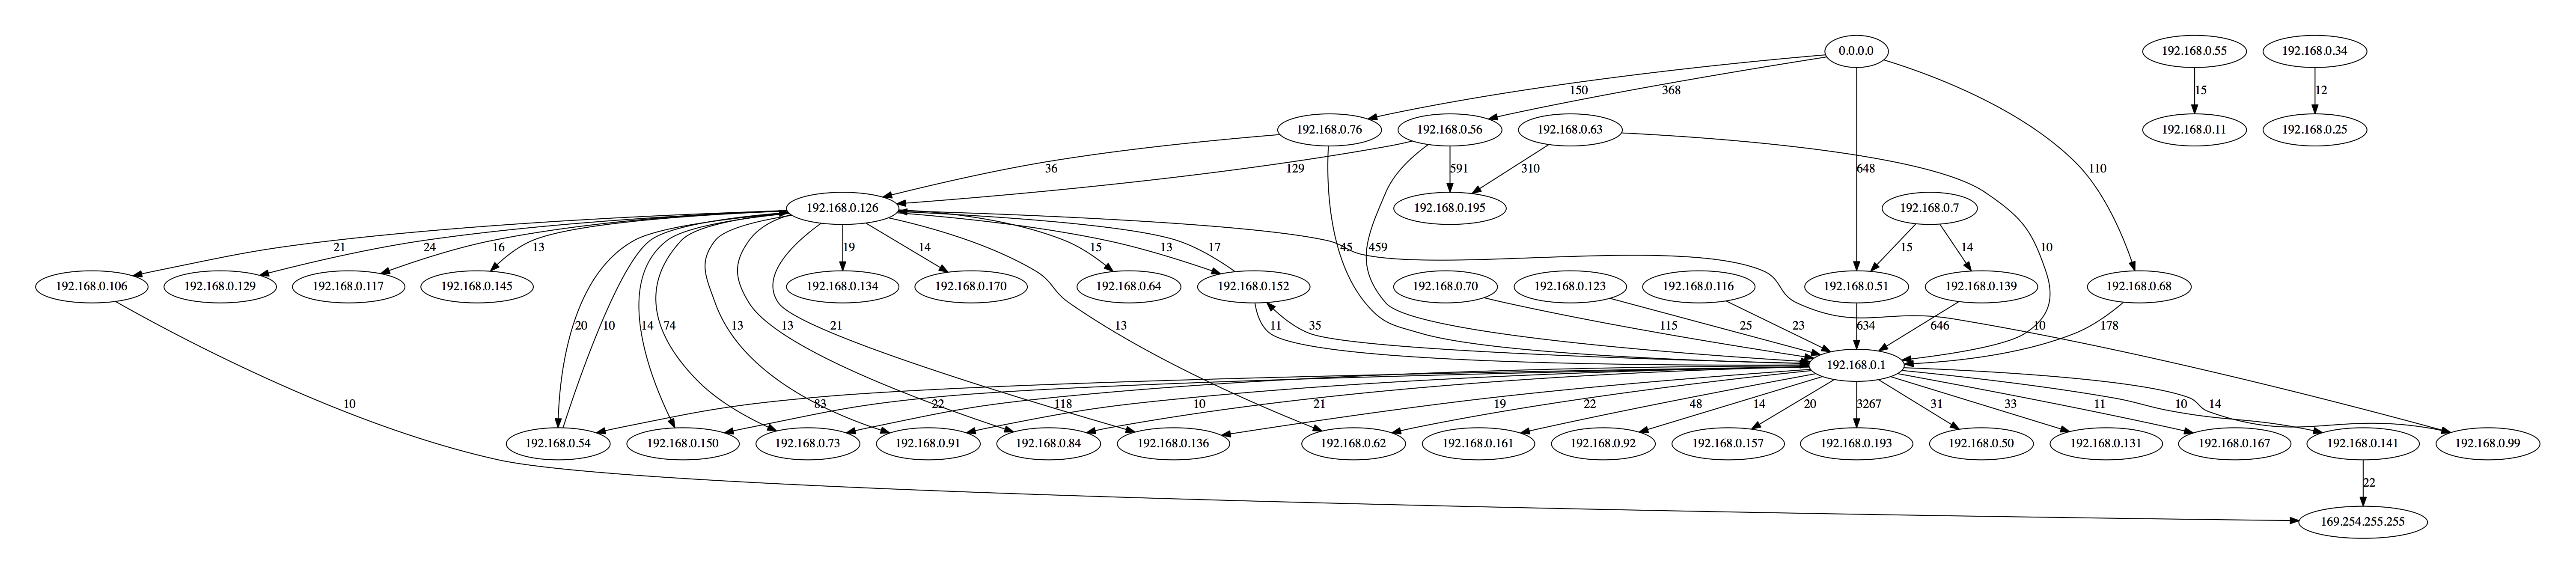
\includegraphics[scale=0.25,angle=90]{graphics/t-work-10000c-10w.png}

A primera vista notamos que hay ciertos nodos que resaltan sobre los demás como el 192.168.0.1 (router), o 192.168.0.126. Si bien la estructura de este digrafo no es un árbol, se nota que hay cierta jerarquía.\newline

Un nodo interesante que resalta es el 169.254.255.255, porque es la única IP no privada que aparece en la red. Analizando este caso en particular, vemos que siempre es buscado por nodos de la red (y éste nunca busca a nadie), lo que nos hace suponer que puede tratarse de un servicio, como un servidor de DNS.\newline

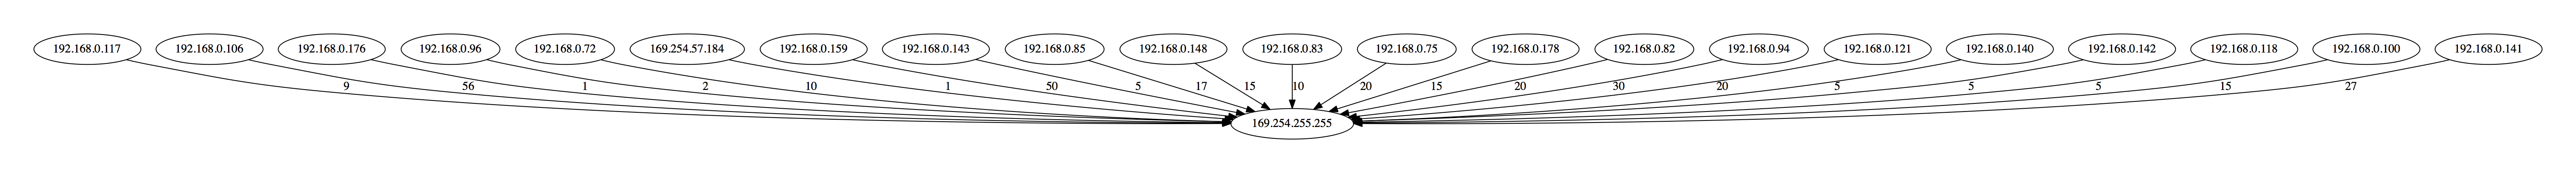
\includegraphics[scale=0.25,clip=true,trim=850 0 870 0]{graphics/t-work-ip-169-254-255-255.png}

Investigando el resto de la captura, notamos que los demás paquetes que recibe son del protocolo NetBIOS Name Service, con lo que podemos afirmar que en este nodo funciona un NetBIOS Server.\newline

Para poder reconocer mejor cuáles son los nodos más importantes de la red veamos el siguiente grafo, donde se estudia toda la muestra pero sólo nos quedamos con aquellos nodos que compartieron más de mil mensajes.\newline

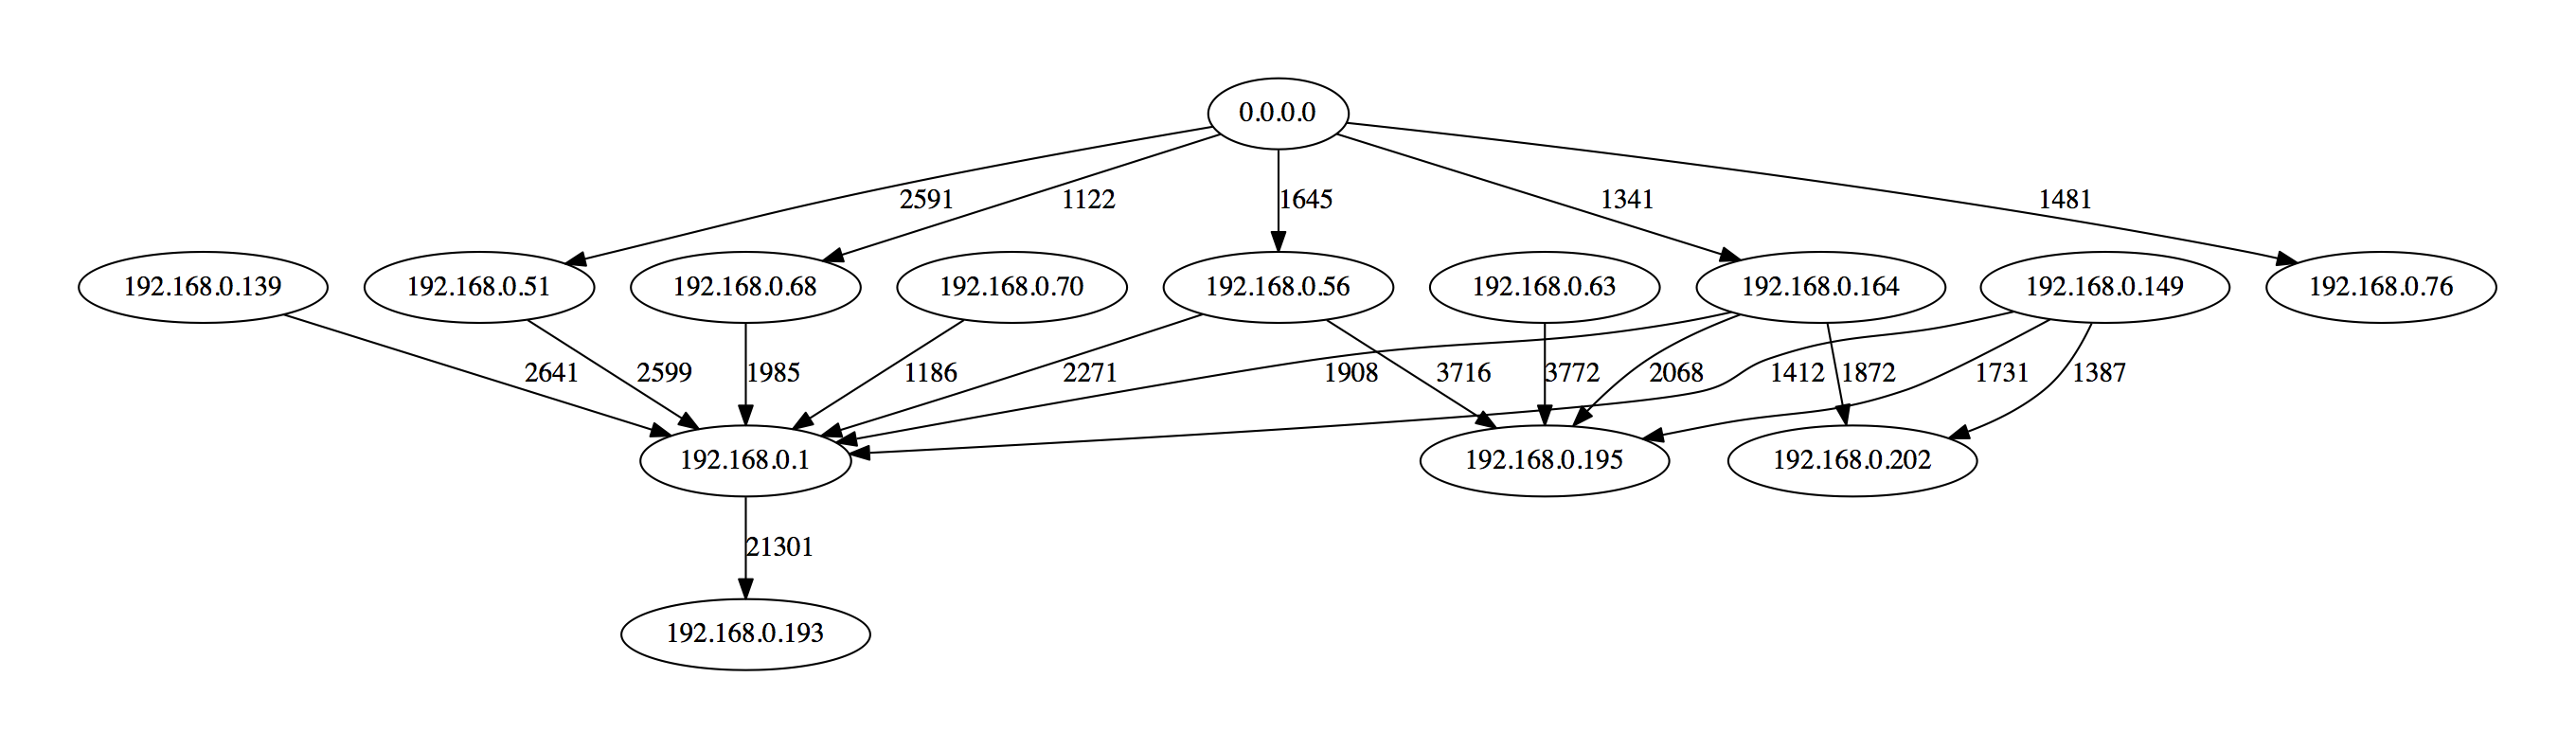
\includegraphics[scale=0.30]{graphics/t-work-all-1000w.png}

Viendo los mensajes ARP de esta manera podemos notar varias cosas. Por un lado que tiene forma de árbol, pero el nodo raíz no es el router, como suponíamos originalmente. Vemos que hay muchos requests ARP que tienen origen en el 0.0.0.0 y como destino diversos nodos de la red, pero ésta no es una IP del rango privado.\newline

Este primer hecho nos llevó a conocer que un ARP con origen 0.0.0.0 es parte de una técnica para detectar direcciones IP duplicadas dentro de una red. En este caso, se estaba queriendo detectar si las direcciones terminadas en 51, 56, 68, 76 ó 164 estaban duplicadas.\newline

\newpage

También nos pareció relevante analizar el router en particular.\newline

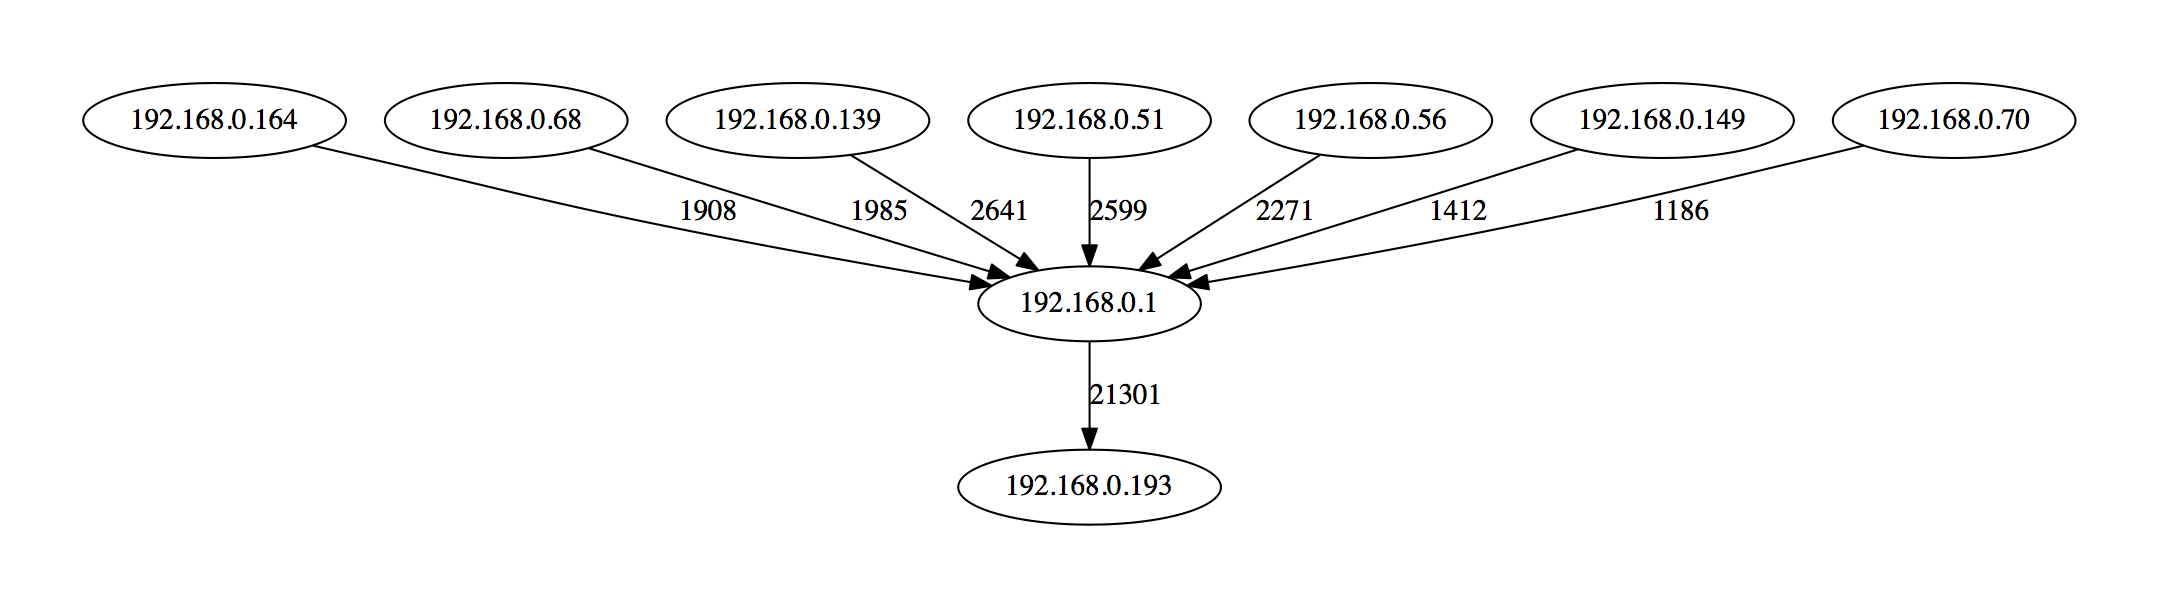
\includegraphics[scale=0.3]{graphics/t-work-router-1000w.png}

Vemos que resulta interesante la gran cantidad de veces que se solicita la IP 192.168.0.193. Para saber más sobre lo que podría estar sucediendo con ese host, revisamos el resto de la captura pero encontramos que no había ningún paquete con esa dirección origen ni destino.\newline

Por esto creemos que podría tratarse de un nodo mal configurado, buscando una IP que ya no existe en la red, lo cual parece en consonancia con la gran cantidad de pedidos ARP que el router le hace.\newline

Finalmente, calculamos la entropía de las fuentes origen y destino: 3.44356252078915 y 4.652923252101102, respectivamente.\newline
